In section \ref{sec:algorithm} we have seen that it is very difficult or even impossible to solve the inverse problem $I \rightarrow \mc D$ directly with a neural network because of multiple designs mapping to a single spectrum. For the algorithm we solved this by adding a conventional optimization method after the network to tune the parameters the network was not able to set correctly. This had some success in the sense that it was able to reproduce know stacks and even some more general functions \note{add this in Appendix?} but this approach is also a big concession because we loose many of the advantages neural networks bring. Conventional optimization methods are way more computationally expensive than a single forward pass in a neural network and more importantly they are very prone to getting stuck in local minima. Having one network being able to solve $I \rightarrow \mc D$ directly would be the best solution.
\\

\indent As this is a well known problem numerous solutions have been proposed. A very interesting route was taken by Liu et al. \cite{Liu2018}. They approach the inverse problem by first solving the forward problem in our case $\mc D \rightarrow I$ and then building a combined network in a kind of tandem structure 
$I \rightarrow \mc D \rightarrow I'$
where the cost function is 
$C = C \qty(I, \, I')$.
This means during training the network is given a target spectrum $I$ and predicts the corresponding design parameters $\mc D$ this design is then fed into the forward model and produces a spectrum $I'$ and the cost function depends on the difference in $I$ and $I'$. This approach completely circumvents the issue of multiple designs mapping to a single spectrum because it only depends on the differences between the target and the produced spectrum. We can already solve the forward problem via the DB and SASA modules as seen in figure \ref{fig:al:combined}.
\\


\indent This combined model can easily be implemented as all the necessary modules are already there but it can not be trained. To understand why we need to go back to the concept of {\hyperref[eq:bg:back_prop]{Backpropagation}}.
During training the gradient of the cost function needs to propagate backwards through the network. To capture this mathematically we will identify the forward model in figure \ref{fig:al:combined} as the last layer $L$ in a combined network. Equation \eqref{eq:bg:back_prop} tells us we need to calculate:

\begin{equation}
    \delta^L_j = \pdv{C}{a^L_j} \ \pdv{a^L_j}{z^L_j}
\end{equation}

The first part $\partial C / \partial{a^L_j}$ is simple and only depends on the cost function. For example using \\
$C_\s{mse} = \sum_j \qty(a_j^L - y_j)^2$
the derivative is 
$\partial{C} / \partial{a^L_j} = 2 \qty(a_j^L - y_j)$
However, the second part 
$\partial{a^L_j} / \partial{z^L_j}$,
the output of the last layer derived by the input to the last layer, is not easily accessible. Maybe not accessible at all if we consider the calls to the database and interpolation that happen during this step. The only way to train this combined tandem model is by replacing the forward model with something where we can access the gradient.

\begin{figure}[H]
    \centering
    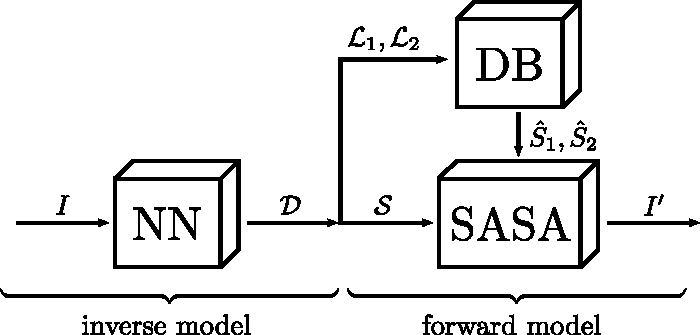
\includegraphics[width=.63\linewidth]{al_combined}
    \caption{A part of the algorithm described in section \ref{sec:algorithm} can be understood as a tandem model 
    $I \rightarrow \mc D \rightarrow I'$.
    This combined model receives a target spectrum and outputs its best reproduction of that spectrum $I'$. The notation is the same as in figure \ref{fig:al:algo}.}
    \label{fig:al:combined}
\end{figure}